\documentclass[a4paper,11pt,french]{report}
\usepackage{CLT2627}
\usepackage{pdfpages}
\makeindex

% Pendant la rédaction : ne décommenter ici que le(s) chapitre(s) en cours d'édition
% pour sauter la mise en page des autres (LaTeX réutilise leurs .aux existants).
% Penser à tout commenter avant de compiler le PDF complet final.
%\includeonly{Chapitres/...}


\begin{document}
\addtocontents{toc}{\protect\hypertarget{toc}{}}
\tableofcontents

\vspace{1em}
\begin{center}
\begin{minipage}{0.9\linewidth}
\footnotesize\itshape
Ce document s'inspire, pour sa structure et une partie de ses exercices et exemples, des travaux de Louis Paternault (\href{https://forge.apps.education.fr/paternaultlouis}{@paternaultlouis}), disponibles sur le dépôt \url{https://forge.apps.education.fr/paternaultlouis/cours-1generale-math-tronccommun} sous licence Creative Commons Attribution - Partage dans les Mêmes Conditions 4.0 International (CC BY-SA 4.0, \url{https://creativecommons.org/licenses/by-sa/4.0/deed.fr}). Les passages directement adaptés de cette source sont signalés individuellement et restent, pour leur part, placés sous cette même licence CC BY-SA 4.0.
\end{minipage}
\end{center}
\vspace{1em}

\part{Analyse de l'information chiffrée}

% !TEX root = ../PolycopiePremiere2627.tex
%%%%%%%%%%%%%%%%%%%%%%%%%%%%%%%%%%%%%%%%%%%%%%%%%%%%%%%%%%%%%%%%%%%%%%%%%%%%%%%%
% Contenu initial repris de Louis Paternault --- http://ababsurdo.fr
%
% Publié sous licence Creative Commons Attribution-ShareAlike 4.0 International (CC BY-SA 4.0)
% http://creativecommons.org/licenses/by-sa/4.0/deed.fr
%%%%%%%%%%%%%%%%%%%%%%%%%%%%%%%%%%%%%%%%%%%%%%%%%%%%%%%%%%%%%%%%%%%%%%%%%%%%%%%%

\chapter{Informations chiffrées}

\section{Nuage de points et Point moyen}

\Dfn{Chaque point d'un \textcolor{J1}{nuage de points} représente un individu, dont les deux caractères étudiés correspondent aux coordonnées de ce point.}

\Dfn{Étant donné un ensemble de points $M_1(x_1;y_1)$, $M_2(x_2;y_2)$, …, $M_n(x_n;y_n)$, on définit le \textcolor{J1}{point moyen} comme le point, noté ici $G$, dont les coordonnées sont la moyenne arithmétique des coordonnées des points de l'ensemble :
\[
    G\left(\frac{x_1+x_2+\cdots+x_n}{n};\frac{y_1+y_2+\cdots+y_n}{n}\right)
\]}

\bigskip

\noindent\textbf{Activité}

Voici le poids à vide (approximatif) et la longueur des voitures les plus vendues en France\footnote{Sources : \emph{Auto moto} et \emph{www.fiches-auto.fr}, compilé par les contributeurs et contributrices de Wikipedia dans l'article \url{https://fr.wikipedia.org/wiki/Voitures_les_plus_vendues_en_France}} dans les années 1960 d'une part, et 2010 d'autre part.

\begin{center}
\begin{tabular}{|M{2.6cm}|M{3cm}|M{2.2cm}|M{2.2cm}|}
    \hline
    \textbf{Année} & \textbf{Modèle} & \textbf{Poids (kg)} & \textbf{Longueur (m)} \tabularnewline
    \hline
    1960 et 1961 & Renault Dauphine & 630 & 3,945 \tabularnewline
    \hline
    1962 à 1965 & Renault 4 & 540 & 3,609 \tabularnewline
    \hline
    1966 & Citroën Ami 6 & 800 & 3,960 \tabularnewline
    \hline
    1967 et 1968 & Renault 4 & 540 & 3,609 \tabularnewline
    \hline
    1969 & Peugeot 204 & 900 & 3,900 \tabularnewline
    \hline
    2010 & Peugeot 207 & 1250 & 4,030 \tabularnewline
    \hline
    2011 et 2012 & Renault Clio III & 1150 & 4,100 \tabularnewline
    \hline
    2013 à 2018 & Renault Clio IV & 1215 & 4,062 \tabularnewline
    \hline
    2019 & Peugeot 208 I & 1100 & 3,972 \tabularnewline
    \hline
\end{tabular}
\end{center}

\begin{enumerate}
    \item Représenter ces données sous la forme d'un nuage de points (dont les abscisses sont le poids, et les ordonnées la taille), en choisissant deux couleurs différentes pour les voitures des années 1960 et 2010.

        \begin{center}
            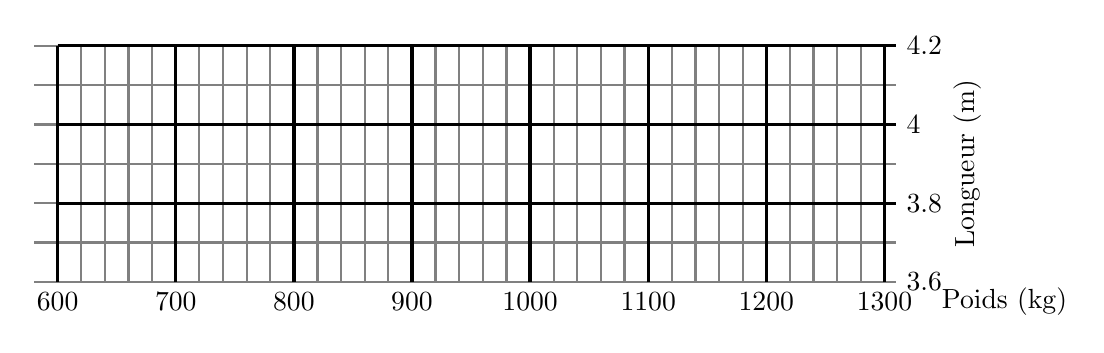
\begin{tikzpicture}[thick, xscale=1.5, yscale=5]
                \draw[gray] (5.8, 3.6) grid[xstep=.2, ystep=.1] (13.1, 4.2);
                \draw[very thick] (6, 3.6) grid[xstep=1, ystep=.2] (13.1, 4.2);
                \foreach \x in {6, 7, ..., 13} {
                    \draw (\x, 3.55) node {\x00};
                }
                \draw (13.4, 3.55) node[anchor=west] {Poids (kg)};
                \foreach \y in {3.6, 3.8, ..., 4.2} {
                    \draw (13.1, \y) node[right]{\y};
                }
                \draw (13.7, 3.9) node[rotate=90]{Longueur (m)};
            \end{tikzpicture}
        \end{center}
    \item Calculer les coordonnées du point moyen de chacune des deux séries, et les représenter sur le graphique.
    \item Commenter : Comment ont évolué le poids et la taille des voitures en cinquante ans ?
\end{enumerate}

\pagebreak

\section{Ajustement affine, Interpolation et Extrapolation}

\noindent\textbf{Activité}

Le nuage de points suivant présente la température mensuelle moyenne mesurée en décembre par une station météorologique aux environs de Lyon, de 1990 à 2025\footnote{Source : \emph{Messages climat — Mensuel}, par Météo France, \url{https://meteo.data.gouv.fr/datasets/6a183217f8648518b7101a3b}.}.

\begin{center}
    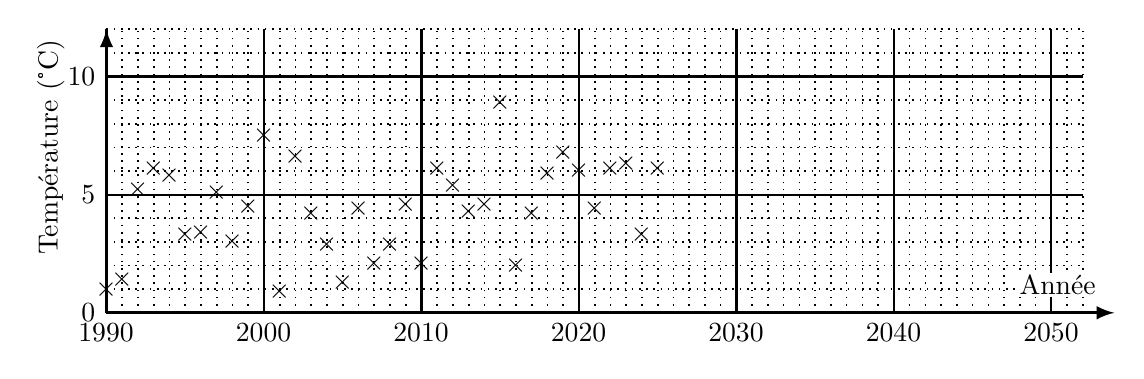
\begin{tikzpicture}[very thick, xscale=20, yscale=.3]
        % C'est très moche comme manière de faire pour tracer un graphique,
        % mais il est tard et je n'arrive pas à faire en sorte que pgfplots fasse ce que je veux.
        \foreach \annee in {1990, 2000, ..., 2050} {
            \draw ({\annee/100}, 0) node[below]{\annee};
            \draw[thick] ({\annee / 100}, 0) -- ++(0, 12);
        }
        \foreach \annee in {1990, 1991, ..., 2052} {
            \draw[semithick, dotted] ({\annee / 100}, 0) -- ++(0, 12);
        }
        \foreach \temperature in {0, 1, ..., 12} {
            \draw[semithick, dotted] (19.9, \temperature) -- (20.52, \temperature);
        }
        \foreach \temperature in {0, 5, ..., 12} {
            \draw (19.9, \temperature) node[left, anchor=east]{\temperature};
            \draw[thick] (19.9, \temperature) -- (20.52, \temperature);
        }
        \draw[-latex] (19.9, 0) -- (20.54, 0) node[above left=.5em, fill=white, inner sep=1pt]{Année};
        \draw[-latex] (19.9, 0) -- (19.9, 12) node[left=2em, rotate=90]{Température (\textdegree C)};
        \foreach \annee / \temperature in {
            1990 / 1,
            1991 / 1.4,
            1992 / 5.2,
            1993 / 6.1,
            1994 / 5.8,
            1995 / 3.3,
            1996 / 3.4,
            1997 / 5.1,
            1998 / 3,
            1999 / 4.5,
            2000 / 7.5,
            2001 / 0.9,
            2002 / 6.6,
            2003 / 4.2,
            2004 / 2.9,
            2005 / 1.3,
            2006 / 4.4,
            2007 / 2.1,
            2008 / 2.9,
            2009 / 4.6,
            2010 / 2.1,
            2011 / 6.1,
            2012 / 5.4,
            2013 / 4.3,
            2014 / 4.6,
            2015 / 8.9,
            2016 / 2,
            2017 / 4.2,
            2018 / 5.9,
            2019 / 6.8,
            2020 / 6,
            2021 / 4.4,
            2022 / 6.1,
            2023 / 6.3,
            2024 / 3.3,
            2025 / 6.1
        }{
            \draw ({\annee / 100}, \temperature) node{$\times$};
        }
    \end{tikzpicture}
\end{center}

Si la tendance se poursuit, quelle sera la température moyenne en décembre 2050 ?

\Dfn{Une \textcolor{J1}{droite d'ajustement} est une droite approchant au mieux un nuage de points.
Plusieurs méthodes existent pour déterminer une telle droite (droite de Mayer, moindres carrés), mais cette année, cette droite sera tracée au jugé.}

\Dfn{
\begin{itemize}
    \item \textcolor{J1}{Interpoler}, c'est déterminer une valeur manquante à l'intérieur d'une série de données.
    \item \textcolor{J1}{Extrapoler}, c'est déterminer une valeur manquante à l'extérieur d'une série de données.
\end{itemize}}

\Exemple{Reprenons le nuage de points de l'activité précédente (températures moyennes de décembre, de 1990 à 2025), et cherchons la température moyenne prévisible en 2050.

\medskip

\textbf{Etape 1} : on calcule les coordonnées du point moyen $G$ du nuage, qui sert de point d'appui pour tracer la droite d'ajustement au jugé.\\
\textcolor{J1}{L'abscisse moyenne des 36 années 1990 à 2025 est $\bar{x}=\dfrac{1990+2025}{2}=2007{,}5$, et la moyenne des 36 températures relevées est $\bar{y}\approx 4{,}4$. Donc $G(2007{,}5\ ;\ 4{,}4)$.}

\medskip

\textbf{Etape 2} : on trace, au jugé, la droite passant par $G$ et suivant au mieux l'allure générale du nuage, puis on la prolonge jusqu'à l'année 2050.\\
\textcolor{J1}{Comme 2050 n'appartient pas à l'intervalle $[1990\ ;\ 2025]$ des années observées, prolonger la droite jusqu'à cette valeur est bien une \emph{extrapolation}.}

\medskip

\textbf{Etape 3} : on lit, sur le graphique, l'ordonnée du point de la droite d'abscisse 2050.\\
\textcolor{J1}{On obtient une température moyenne prévisible d'environ 7\textdegree C en décembre 2050 --- un résultat approximatif, puisqu'il dépend de la droite tracée à main levée.}
}

\section{Tableau croisé d'effectifs}

\Dfn{Un \textcolor{J1}{tableau croisé d'effectifs} (ou table de contingence) présente les effectifs obtenus en croisant deux caractères observés sur une même population. Les totaux inscrits en marge de chaque ligne et de chaque colonne, appelés \textcolor{J1}{effectifs marginaux}, donnent, pour chaque modalité d'un des deux caractères, l'effectif total toutes modalités de l'autre caractère confondues.}

\bigskip

\Exemple{Dans un lycée, on interroge les élèves de première sur leur choix de suivre (ou non) l'enseignement de spécialité Mathématiques. Voici les effectifs obtenus, selon le sexe.

\begin{center}
\begin{tabular}{|l|c|c|c|}
    \hline
     & \textbf{Filles} & \textbf{Garçons} & \textbf{Total} \\
    \hline
    \textbf{Suivent la spécialité Maths} & 40 & 60 & \textcolor{J1}{100} \\
    \hline
    \textbf{Ne suivent pas la spécialité} & 80 & 40 & \textcolor{J1}{120} \\
    \hline
    \textbf{Total} & \textcolor{J1}{120} & \textcolor{J1}{100} & \textcolor{J1}{220} \\
    \hline
\end{tabular}
\end{center}

\medskip

\textbf{Etape 1} : on complète les effectifs marginaux en additionnant chaque ligne, puis chaque colonne (le total général s'obtient de deux façons --- en sommant les totaux de lignes, ou ceux des colonnes --- ce qui permet de vérifier le tableau).\\
\textcolor{J1}{Ligne « spécialité » : $40+60=100$. Ligne « pas de spécialité » : $80+40=120$. Colonne « Filles » : $40+80=120$. Colonne « Garçons » : $60+40=100$. Total général : $100+120=120+100=220$.}

\medskip

\textbf{Etape 2} : quelle proportion des élèves suivant la spécialité Mathématiques sont des filles ?\\
\textcolor{J1}{Parmi les 100 élèves qui suivent la spécialité, 40 sont des filles, soit une proportion de $\dfrac{40}{100}=0{,}4=40\,\%$.}
}

\section{Diagrammes}

\Prp{Dans un diagramme circulaire, les angles de chacune des sections sont \textcolor{J1}{proportionnels} aux effectifs correspondants.}

\Exemple{
    \begin{multicols}{2}
    Le tableau ci-contre représente le temps quotidien passé à réaliser des tâches ménagères, par les hommes et les femmes\footnote{Source : \emph{Femmes et hommes - Regards sur la parité}, \textsc{Insee}, 2012, \url{https://www.insee.fr/fr/statistiques/1372773?sommaire=1372781&q=taches+domestiques}}.

        \columnbreak

        \begin{center}
            \begin{tabular}{|r|c|c|c|}
                \hline
                & \textbf{1986} & \textbf{1999} & \textbf{2010} \\
                \hline
                Hommes & 2h07 & 2h13 & 2h13 \\
                \hline
                Femmes & 5h07 & 4h36 & 4h01 \\
                \hline
            \end{tabular}
        \end{center}
    \end{multicols}

    Représentons, sous la forme d'un diagramme circulaire, la répartition entre hommes et femmes du temps consacré aux tâches ménagères en 2010.

    \medskip

    \textbf{Etape 1} : on convertit les deux durées dans la même unité (les minutes), puis on calcule leur somme.\\
    \textcolor{J1}{Hommes : $2\text{h}13 = 133$ min. Femmes : $4\text{h}01=241$ min. Total : $133+241=374$ min.}

    \medskip

    \textbf{Etape 2} : d'après la propriété précédente, l'angle de chaque secteur est proportionnel à la durée qu'il représente ; on applique un produit en croix sur $360$\textdegree.\\
    \textcolor{J1}{Secteur « Hommes » : $\dfrac{133}{374}\times 360 \approx 128$\textdegree. Secteur « Femmes » : $\dfrac{241}{374}\times 360 \approx 232$\textdegree\ (on vérifie bien que $128+232=360$).}

    \medskip

    \textbf{Etape 3} : on reporte ces deux angles au rapporteur pour tracer le diagramme circulaire.

    \begin{center}
        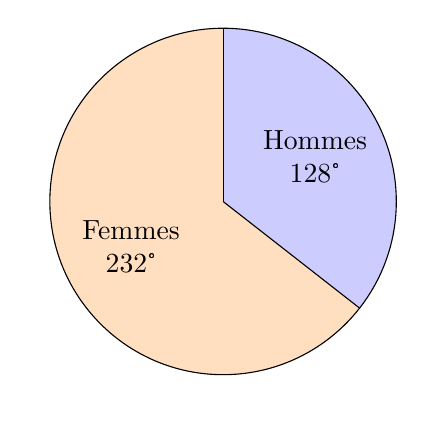
\begin{tikzpicture}
            \fill[blue!20] (0,0) -- (90:2.2) arc (90:-38:2.2) -- cycle;
            \fill[orange!25] (0,0) -- (-38:2.2) arc (-38:-270:2.2) -- cycle;
            \draw (0,0) circle (2.2);
            \draw (0,0) -- (90:2.2);
            \draw (0,0) -- (-38:2.2);
            \node[align=center] at (26:1.3) {Hommes\\128\textdegree};
            \node[align=center] at (206:1.3) {Femmes\\232\textdegree};
        \end{tikzpicture}
    \end{center}
}


\part{Phénomènes aléatoires}

% !TEX root = ../PolycopiePremiere2627.tex
%%%%%%%%%%%%%%%%%%%%%%%%%%%%%%%%%%%%%%%%%%%%%%%%%%%%%%%%%%%%%%%%%%%%%%%%%%%%%%%%
% Contenu initial repris de Louis Paternault --- http://ababsurdo.fr
%
% Publié sous licence Creative Commons Attribution-ShareAlike 4.0 International (CC BY-SA 4.0)
% http://creativecommons.org/licenses/by-sa/4.0/deed.fr
%%%%%%%%%%%%%%%%%%%%%%%%%%%%%%%%%%%%%%%%%%%%%%%%%%%%%%%%%%%%%%%%%%%%%%%%%%%%%%%%

\chapter{Probabilités conditionnelles}

\section{Fréquences marginales, fréquences conditionnelles}

\Dfn{Dans un tableau croisé d'effectifs :
\begin{itemize}
    \item la valeur à l'intersection d'une ligne et d'une colonne est le nombre d'individus présentant simultanément les deux caractères ;
    \item on appelle \textcolor{J1}{effectif marginal} l'effectif d'une sous-population qui ne dépend que d'un seul caractère. Ces effectifs sont représentés dans la ligne « Total » ou la colonne « Total » ;
    \item la \textcolor{J1}{fréquence marginale} d'une valeur est le quotient :
    \[\dfrac{\text{Effectif marginal}}{\text{Effectif total}}\]
    \item la \textcolor{J1}{fréquence conditionnelle} de la valeur $x_i$ sachant $y_j$ est le quotient :
    \[\dfrac{\text{Effectif présentant les valeurs $x_i$ et $y_j$}}{\text{Effectif marginal de la valeur $y_j$}}\]
\end{itemize}}

\Exemple{Un nouveau test a été développé pour détecter une maladie, et on souhaite évaluer son efficacité. On prend un échantillon représentatif de \numprint{1000} personnes dans la population, dont on sait par ailleurs si elles sont malades ou non, et on leur fait passer le test. On obtient les résultats suivants (où « diagnostic positif » signifie que le test a détecté la maladie, peut-être à tort).
\begin{center}
    \begin{tabular}{|M{3.4cm}|M{1.8cm}|M{1.8cm}|M{1.8cm}|}
        \hline
        & \textbf{Malade} & \textbf{Saine} & \textbf{Total} \tabularnewline
        \hline
        Diagnostic positif & 19 & 79 & \tabularnewline
        \hline
        Diagnostic négatif & & 901 & \tabularnewline
        \hline
        Total & & & \tabularnewline
        \hline
    \end{tabular}
\end{center}

\begin{enumerate}
    \item Complétez le tableau.
    \item Combien de personnes malades ont obtenu un test négatif ?
    \item Calculez la fréquence marginale de personnes malades dans la population.
    \item Calculez la fréquence de diagnostics corrects. Le test est-il fiable ?
    \item Calculez la fréquence conditionnelle de personnes malades sachant que le diagnostic est positif.
\end{enumerate}}

\section{Probabilités conditionnelles}

\Dfn[Rappels]{Étant donnés deux évènements $A$ et $B$ d'un univers $\Omega$ :
\begin{itemize}
    \item l'intersection de $A$ et $B$, notée $A\cap B$, est \textcolor{J1}{l'ensemble des éléments qui appartiennent à la fois à $A$ et à $B$} ;
    \item l'union de $A$ et $B$, notée $A\cup B$, est \textcolor{J1}{l'ensemble des éléments qui appartiennent à $A$, ou à $B$, ou aux deux à la fois} ;
    \item le contraire de $A$, noté $\overline{A}$, est \textcolor{J1}{l'ensemble des issues de l'univers qui n'appartiennent pas à $A$}.
\end{itemize}}

\Exemple{On considère les élèves de cette classe, et :
\begin{itemize}
    \item $A$ : « l'ensemble des garçons » ;
    \item $B$ : « l'ensemble des personnes portant des lunettes ».
\end{itemize}
Alors :
\begin{itemize}
    \item $A\cup B$ est : \textcolor{J1}{l'ensemble des garçons à lunettes}.
    \item $\overline{B}$ est : \textcolor{J1}{l'ensemble des personnes sans lunettes}.
    \item $A\cap\overline{B}$ est : \textcolor{J1}{l'ensemble des garçons sans lunettes}.
\end{itemize}}

\Dfn[Rappel]{On choisit de manière équiprobable un individu au hasard dans une population, et on considère un évènement $A$. Alors :
\[
    P(A)=\textcolor{J1}{\dfrac{\text{Nombre de cas favorables}}{\text{Nombre de cas possibles}}}
\]}

\Exemple{Pour vérifier la qualité d'une chaîne de montage d'aspirateurs, une équipe vérifie leur fonctionnement : sur 67 aspirateurs étudiés, 3 ne fonctionnent pas.

On choisit un aspirateur au hasard à la sortie de cette chaîne de montage. Quelle est la probabilité qu'il ne fonctionne pas ?}

\Dfn{Soient $A$ et $B$ deux évènements d'une expérience aléatoire, tels que $P(B)\neq0$.

On appelle \textcolor{J1}{probabilité conditionnelle de $A$ sachant $B$}, ou « probabilité que $A$ soit réalisé sachant que $B$ est réalisé », le nombre :
\[P_B\left( A \right)=\dfrac{\mathrm{card}(A\cap B)}{\mathrm{card}(B)}=\dfrac{P\left( A\cap B \right)}{P\left( B \right)}\]}

\Exemple{On lance un dé équilibré à six faces, et on observe le résultat obtenu. On note $P$ : « le résultat est pair », et $Q$ : « le résultat est supérieur ou égal à quatre ».
\begin{enumerate}
    \item Calculer la probabilité que le résultat soit pair.
    \item Calculer la probabilité que le résultat soit pair, sachant qu'il est supérieur ou égal à 4.
\end{enumerate}}

\Dfn{Deux évènements $A$ et $B$ (avec $P(B)\neq0$) sont dits \textcolor{J1}{indépendants} si $P_B(A)=P(A)$.}

\Prp{Deux évènements $A$ et $B$ sont \textcolor{J1}{indépendants} si et seulement si $P(A\cap B)=P(A)\times P(B)$.}

\Exemple[Inspiré du sujet 0 du baccalauréat d'enseignement spécifique, sujet 2, 2025]{
% Dactylographié par l'APMEP. Merci à elles et eux.
Dans un lycée comptant $\numprint{2000}$ élèves, on donne la répartition des effectifs suivant le sexe et le choix de la LV1.

\begin{center}
    \begin{tabular}{|M{2.6cm}|M{2cm}|M{2cm}|}
        \hline
        & \textbf{Fille} & \textbf{Garçon} \tabularnewline
        \hline
        Anglais & 712 & 728 \tabularnewline
        \hline
        Autre LV1 & 288 & 272 \tabularnewline
        \hline
    \end{tabular}
\end{center}

\begin{enumerate}
    \item Un élève affirme « Dans ce lycée, il y a autant de filles que de garçons ». A-t-il raison ? Justifier.
\end{enumerate}

On choisit au hasard, de manière équiprobable, un élève dans ce lycée.

On considère les évènements suivants :

$F$ : « l'élève est une fille » ;

$A$ : « l'élève a choisi Anglais pour LV1 ».

Dans les questions qui suivent, on donnera les résultats sous forme d'une fraction qu'il n'est pas demandé de simplifier.

\begin{enumerate}[resume]
    \item Déterminer la probabilité de l'évènement $A \cap F$.
    \item Déterminer la probabilité de l'évènement $A$ sachant que l'évènement $F$ est réalisé.
    \item Les évènements $A$ et $F$ sont-ils indépendants ? Justifier.
    \item On sait que l'élève choisi est un garçon. On considère l'affirmation suivante :

    « La probabilité qu'il ait choisi Anglais pour LV1 est plus de trois fois plus grande que la probabilité qu'il n'ait pas choisi Anglais pour LV1 ».

    Cette affirmation est-elle vraie ? Justifier.
\end{enumerate}}

\pagebreak

\section{Répétition d'expériences aléatoires}

\Prp{On peut modéliser la succession d'expériences aléatoires par un arbre de probabilités (ou arbre pondéré) respectant les règles suivantes.
\begin{itemize}
    \item La somme des probabilités des branches issues d'un nœud est égale à 1.
    \item La probabilité d'une issue d'un chemin est égale au produit des probabilités rencontrées sur le chemin.
    \item La probabilité d'un évènement est égale à la somme des probabilités des issues qui le composent.
\end{itemize}}

\Exemple[Inspiré du sujet 0 du baccalauréat d'enseignement spécifique, sujet 3, 2025]{
% Dactylographié par Denis Vergès, de l'APMEP. Merci à lui.
Un village propose aux participants de la fête du sport deux épreuves : une randonnée et un cross. Il n'est pas possible de s'inscrire aux deux épreuves à la fois.
On dispose des informations suivantes :
\begin{itemize}
    \item $90\,\%$ des participants ont choisi la randonnée, parmi eux, $5\,\%$ sont licenciés dans un club ;
    \item $10\,\%$ des participants ont choisi le cross, parmi eux, $40\,\%$ sont licenciés dans un club.
\end{itemize}

Un journaliste interroge un participant au hasard, et on considère les évènements suivants :

$R$ : « Le participant a choisi la randonnée » ;

$L$ : « Le participant est licencié dans un club ».

\begin{enumerate}
    \item Par simple lecture de l'énoncé, indiquer :
    \begin{enumerate}
        \item La probabilité que le participant interrogé soit licencié dans un club sachant qu'il a choisi la randonnée.
        \item La probabilité que le participant interrogé soit licencié dans un club sachant qu'il a choisi le cross.
    \end{enumerate}
\end{enumerate}

\begin{enumerate}[resume]
    \item Représenter la situation par un arbre de probabilité.
    \item
    \begin{enumerate}
        \item Déterminer la probabilité que le participant interrogé ait choisi le cross et soit licencié dans un club.
        \item Vérifier que la probabilité que le participant interrogé soit licencié dans un club est égale à $\dfrac{850}{10000}$, soit $8,5\,\%$.
    \end{enumerate}
    \item Le journaliste interroge un participant licencié dans un club. Déterminer la probabilité que ce participant ait choisi le cross.
\end{enumerate}}


\part{Phénomènes d'évolution}

% !TEX root = ../PolycopiePremiere2627.tex
%%%%%%%%%%%%%%%%%%%%%%%%%%%%%%%%%%%%%%%%%%%%%%%%%%%%%%%%%%%%%%%%%%%%%%%%%%%%%%%%
% Contenu initial repris de Louis Paternault --- http://ababsurdo.fr
%
% Publié sous licence Creative Commons Attribution-ShareAlike 4.0 International (CC BY-SA 4.0)
% http://creativecommons.org/licenses/by-sa/4.0/deed.fr
%%%%%%%%%%%%%%%%%%%%%%%%%%%%%%%%%%%%%%%%%%%%%%%%%%%%%%%%%%%%%%%%%%%%%%%%%%%%%%%%

\chapter{Fonction affine}

\Dfn{Une \emph{fonction affine} est une fonction pouvant être exprimée sous la forme $x\mapsto ax+b$, où $a$ et $b$ sont des nombres réels. Elle est définie sur \textcolor{J1}{$\mathbb R$}.}

\Dfn{La courbe d'une fonction affine $f:x\mapsto ax+b$ est une droite, dont :
\begin{itemize}
    \item $a$ est \textcolor{J1}{le coefficient directeur}.
    \item $b$ est \textcolor{J1}{l'ordonnée à l'origine}.
\end{itemize}}

\Prp{Soit $f$ une fonction affine.
\begin{itemize}
    \item Soient $A$ et $B$ deux points de sa courbe représentative. Alors le coefficient directeur est donné par la formule :
    \(\dfrac{y_B-y_A}{x_B-x_A}\).
    \item Soient deux nombres $a$ et $b$ distincts. Alors le coefficient directeur est donné par la formule :
    \(\dfrac{f(b)-f(a)}{b-a}\).
\end{itemize}}

\Exemple{
\begin{enumerate}
    \item Déterminer le coefficient directeur de la fonction affine dont la droite passe par les points $A(2;-7)$ et $B(7;0)$.
    \item Déterminer le coefficient directeur de la fonction affine $f$ telle que $f(-8)=3$ et $f(2)=0$.
\end{enumerate}}

\Prp{Soit $f:x\mapsto ax+b$ une fonction affine. Alors :
\begin{itemize}
    \item si $a<0$, alors la fonction est \textcolor{J1}{strictement décroissante} ;
    \item si $a=0$, alors la fonction est \textcolor{J1}{constante} ;
    \item si $a>0$, alors la fonction est \textcolor{J1}{strictement croissante}.
\end{itemize}}

\Dfn{Une fonction affine permet de modéliser la croissance d'un phénomène linéaire continu :
\begin{itemize}
    \item linéaire : le taux d'accroissement de la fonction est constant ;
    \item continu (par opposition à \emph{discret}) : le phénomène peut être étudié sur un intervalle (plutôt que, par exemple, sur l'ensemble des entiers).
\end{itemize}}

\Exemple{Dire si les phénomènes suivants sont linéaires ou non, continus ou discrets.
\begin{enumerate}
    \item Évolution de l'aire d'un carré en fonction de la longueur d'un de ses côtés.
    \item Évolution de la température d'une casserole d'eau sur le feu en fonction du temps.
    \item Évolution de la somme d'argent dans une tirelire dans laquelle on ajoute 10 € tous les mois.
    \item Évolution de la TVA d'un article en fonction de son prix.
\end{enumerate}}

% !TEX root = ../PolycopiePremiere2627.tex
%%%%%%%%%%%%%%%%%%%%%%%%%%%%%%%%%%%%%%%%%%%%%%%%%%%%%%%%%%%%%%%%%%%%%%%%%%%%%%%%
% Contenu initial repris de Louis Paternault --- http://ababsurdo.fr
%
% Publié sous licence Creative Commons Attribution-ShareAlike 4.0 International (CC BY-SA 4.0)
% http://creativecommons.org/licenses/by-sa/4.0/deed.fr
%%%%%%%%%%%%%%%%%%%%%%%%%%%%%%%%%%%%%%%%%%%%%%%%%%%%%%%%%%%%%%%%%%%%%%%%%%%%%%%%

\chapter{Suites arithmétiques}

\noindent\textbf{Activité}

On définit la suite $u$ à l'aide des schémas suivants (à chaque étape, on compte le nombre de cases de la « couronne » ajoutée au schéma existant).

\begin{minipage}{.3\linewidth}
    \begin{tikzpicture}[scale=.4,very thick]
        \draw[dashed, gray] (-4, -4) grid (6, 5);
        % u1
        \draw (0, 0) rectangle (2, 1);
        % u2
        \draw (-1, -1) rectangle (3, 2);
        \draw[darkgray, arrows={Circle[scale=.5]-}] (0.8, 0.5) -- (-3, 0) node[black, anchor=east, fill=white, inner sep=1pt]{$u(0)=2$};
        \draw[darkgray, arrows={Circle[scale=.5]-}] (0.3, 1.5) -- (-3, 1.5) node[black, anchor=east, fill=white, inner sep=1pt]{$u(1)=10$};
        \draw[darkgray, arrows={Circle[scale=.5]-}] (-0.2, 2.5) -- (-3, 3) node[black, anchor=east, fill=white, inner sep=1pt]{$u(2)=18$};
        % u3
        \draw (-2, -2) rectangle (4, 3);
    \end{tikzpicture}
\end{minipage}%
\hfill%
\begin{minipage}{.6\linewidth}
    \begin{enumerate}
        \item Compléter :
        \begin{center}
            \begin{tabular}{c|c|c}
                $u(4)=\textcolor{J1}{34}$  & $u(\textcolor{J1}{12})=98$ & $u(0)=\textcolor{J1}{2}$ \\[5mm]
                $u(5)=\textcolor{J1}{42}$  &                & $u(-2)=\textcolor{J1}{-14}$ \\[5mm]
                $u(13)=\textcolor{J1}{106}$ &                & $u(4,5)=\textcolor{J1}{38}$ \\[5mm]
            \end{tabular}
        \end{center}
    \end{enumerate}
\end{minipage}

\begin{enumerate}[resume]
    \item On affirme que $u(26)=210$. Compléter :

    \begin{tabularx}{\linewidth}{XXX}
        $u(27)=\textcolor{J1}{218}$ ;&
        $u(25)=\textcolor{J1}{202}$ ;&
        $u(126)=\textcolor{J1}{1010}$.\\
    \end{tabularx}
    \item Pour une certaine valeur de $n$ inconnue, on a : $u(n)=530$. Compléter :

    \begin{tabularx}{\linewidth}{XX}
        $u(n+1)=\textcolor{J1}{538}$ ;&
        $u(n)+1=\textcolor{J1}{531}$ ;\\
        $u(n-1)=\textcolor{J1}{522}$ ;&
        $u(n+2)=\textcolor{J1}{546}$.\\
    \end{tabularx}
    \item
    \begin{enumerate}
        \item Sur le graphique suivant, placer les points correspondant à $u(0)$, $u(1)$ jusqu'à $u(5)$.
        \begin{center}
            \begin{tikzpicture}[xscale=1,yscale=.09,very thick]
                \draw[-latex] (0, 0) -- (8.5, 0);
                \draw[-latex] (0, 0) -- (0, 75);
                \draw[dotted] (0, 0) grid[xstep=1, ystep=5] (8, 70);
                \draw (0, 0) node[below left]{$0$};
                \foreach \x in {1, 2, ..., 8}{
                    \draw (\x, 0) node[below]{$\x$};
                }
                \foreach \y in {10, 20, ..., 70}{
                    \draw (0, \y) node[left]{$\y$};
                }
                \foreach \n/\v in {0/2, 1/10, 2/18, 3/26, 4/34, 5/42}{
                    \draw (\n, \v) node{\textcolor{J1}{$\times$}};
                }
            \end{tikzpicture}
        \end{center}
        \item Compléter par lecture graphique :

        \begin{tabularx}{\linewidth}{XXX}
            $u(6)=\textcolor{J1}{50}$ ;&
            $u(7)=\textcolor{J1}{58}$ ;&
            $u(8)=\textcolor{J1}{66}$.\\
        \end{tabularx}
    \end{enumerate}
\end{enumerate}

\pagebreak

\section{Suites numériques}

\Dfn{On appelle \textcolor{J1}{suite numérique} une suite finie ou infinie de nombres, appelés \textcolor{J1}{termes de la suite}. Cette suite est habituellement notée $u$, $v$ ou $w$. Le premier terme est le plus souvent $u(0)$ ou $u(1)$, et pour un nombre entier $n$, $u(n)$ est \textcolor{J1}{le terme de rang $n$}.

$u(n+1)$ est le terme qui suit $u(n)$, et $u(n-1)$ est le terme qui précède $u(n)$.}

\Exemple{\label{ex:termes}
\begin{enumerate}
    \item On considère $u$ la suite de premier terme $u(0)=8$, et dont chaque terme (sauf le premier) est égal à la moitié du précédent.

    \begin{enumerate}[label=\alph*)]
        \item Calculer $u(3)$ : \textcolor{J1}{$u(3)=1$.}
        \item Calculer le 5\ieme{} terme : \textcolor{J1}{le 1\ier{} terme est $u(0)$, donc le 5\ieme{} terme est $u(4)=0,5$.}
        \item Calculer le terme de rang 2 : \textcolor{J1}{$u(2)=2$.}
    \end{enumerate}
    \item On considère $v$ la suite définie pour tout nombre entier $n\geq1$ par $v(n)=2n^2-3$.

    \begin{enumerate}[label=\alph*)]
        \item Calculer $v(3)$ : \textcolor{J1}{$v(3)=2\times3^2-3=15$.}
        \item Calculer le 4\ieme{} terme : \textcolor{J1}{le 1\ier{} terme est $v(1)$, donc le 4\ieme{} terme est $v(4)=29$.}
        \item Calculer le terme de rang 2 : \textcolor{J1}{$v(2)=5$.}
    \end{enumerate}
    \item On considère $w$ la suite définie par :
    \begin{equation*}
        \left\{\begin{aligned}
            w(0) &= 5\\
            w(n+1) &= 2w(n)-4 \text{ pour tout $n$ entier positif.}\\
        \end{aligned}\right.
    \end{equation*}

    \begin{enumerate}[label=\alph*)]
        \item Calculer $w(3)$ : \textcolor{J1}{$w(1)=6$, $w(2)=8$, $w(3)=12$.}
        \item Calculer le 4\ieme{} terme : \textcolor{J1}{le 1\ier{} terme est $w(0)$, donc le 4\ieme{} terme est $w(3)=12$.}
        \item Calculer le terme de rang 2 : \textcolor{J1}{$w(2)=8$.}
    \end{enumerate}
\end{enumerate}}

\ANoter{Le module \emph{Suites} de la calculatrice permet de manipuler les suites.}

\Exemple{À la calculatrice, reprendre les suites $u$, $v$, $w$ de l'exemple \ref{ex:termes}, et calculer $u(100)$, $v(100)$, $w(100)$.

\textcolor{J1}{$u(100)=8\times0,5^{100}\approx6,3\times10^{-30}$ ; $v(100)=2\times100^2-3=\numprint{19997}$ ; $w(100)=4+2^{100}\approx1,268\times10^{30}$.}}

\Dfn[Variations]{Une suite $u$ est dite :
\begin{itemize}
    \item \textcolor{J1}{croissante} si chaque terme est plus grand que le précédent : ${u(n+1)\geq u(n)}$ ;
    \item \textcolor{J1}{constante} si chaque terme est égal au précédent : $u(n+1)= u(n)$ ;
    \item \textcolor{J1}{décroissante} si chaque terme est plus petit que le précédent : ${u(n+1)\leq u(n)}$.
\end{itemize}}

\Dfn[Représentation graphique]{La représentation graphique d'une suite $u$ est le nuage de points de coordonnées $\left( n;u(n) \right)$.}

\Exemple{\label{ex:graphRecurrente}
On définit la suite $u$ sur $\mathbb{N}$ par :
\begin{equation*}
    \left\{\begin{aligned}
        u(0) &= 0,5\\
        u(n+1) &= 0,75u(n)+1 \text{ pour tout $n$ entier positif.}\\
    \end{aligned}\right.
\end{equation*}
\begin{enumerate}
    \item À l'aide de la calculatrice, déterminer les onze premiers termes de la suite (arrondir au dixième).

    \textcolor{J1}{$u(0)=0,5$ ; $u(1)\approx1,4$ ; $u(2)\approx2,0$ ; $u(3)\approx2,5$ ; $u(4)\approx2,9$ ; $u(5)\approx3,2$ ; $u(6)\approx3,4$ ; $u(7)\approx3,5$ ; $u(8)\approx3,6$ ; $u(9)\approx3,7$ ; $u(10)\approx3,8$.}
    \item Tracer la suite sur le graphique ci-dessous.
    \begin{center}
        \begin{tikzpicture}[scale=1,very thick]
            \begin{axis}[
                    yscale=.5,
                    xscale=1.6,
                    xmin=0,
                    xmax=10,
                    ymin=0,
                    ymax=4,
                    ultra thick,
                    axis lines=middle,
                    enlargelimits=upper,
                    minor y tick num=3,
                    xtick={0, 1, ..., 10},
                    ytick={0, 1, ..., 4},
                    major grid style={black, thick},
                    grid=both,
                    clip=false,
                ]
                \draw (axis cs:0, 0) node[below left]{$0$};
                \addplot[only marks, mark=x, J1, thick] coordinates {
                    (0,0.5) (1,1.4) (2,2.0) (3,2.5) (4,2.9) (5,3.2)
                    (6,3.4) (7,3.5) (8,3.6) (9,3.7) (10,3.8)
                };
            \end{axis}
        \end{tikzpicture}%
    \end{center}
\end{enumerate}}

\Exemple{Par lecture graphique, conjecturer le sens de variation de la suite $u$ de l'exemple précédent.

\textcolor{J1}{La suite $u$ semble croissante.}}

\section{Suites arithmétiques}

\noindent\textbf{Activité}

L'activité d'une entreprise étant florissante, en moyenne 7 nouveaux employés ont été embauchés chaque année. En 2021, elle comptait 38 employés, et on suppose que cette progression va se poursuivre dans les années à venir.

On appelle $u(n)$ le nombre d'employés l'année $2021+n$.

\begin{enumerate}
    \item Donner les cinq premiers termes de la suite : \textcolor{J1}{$u(0)=38$ ; $u(1)=45$ ; $u(2)=52$ ; $u(3)=59$ ; $u(4)=66$.}
    \item Combien y aura-t-il d'employés en 2035 ? \textcolor{J1}{$2035=2021+14$, donc $u(14)=38+7\times14=136$ employés.}
    \item Exprimer $u(n+1)$ en fonction de $u(n)$, pour tout $n\in\mathbb{N}$ : \textcolor{J1}{$u(n+1)=u(n)+7$.}
\end{enumerate}

\bigskip

Une suite est arithmétique si on passe au terme suivant en ajoutant (ou soustrayant) toujours le même nombre.

\Dfn{Une suite $u$ est dite \textcolor{J1}{arithmétique} s'il existe un réel $r$, appelé \textcolor{J1}{raison}, tel que pour tout $n\in\mathbb{N}$, on ait : \textcolor{J1}{$u(n+1)=u(n)+r$}.

Habituellement, une suite arithmétique est définie par la donnée de \textcolor{J1}{son premier terme et sa raison}.}

\Exemple{\label{ex:calcul}
\begin{enumerate}
    \item Donner les cinq premiers termes de la suite arithmétique $u$ de premier terme $u(0)=13$ et de raison \numprint{-2.5} : \textcolor{J1}{$u(0)=13$ ; $u(1)=10,5$ ; $u(2)=8$ ; $u(3)=5,5$ ; $u(4)=3$.}
    \item La suite $v$ est arithmétique, et on sait que $v(3)=1$ et $v(4)=3$. Déterminer la raison, puis calculer $v(5)$, $v(8)$, et $v(2)$ : \textcolor{J1}{$r=v(4)-v(3)=2$, donc $v(5)=v(4)+r=5$, $v(8)=v(4)+4r=11$ et $v(2)=v(3)-r=-1$.}
\end{enumerate}}

\Exemple{\label{ex:graphArithmetique}
Représenter graphiquement (de couleur différente) les deux suites de l'exemple \ref{ex:calcul}. Que remarquez-vous ?
\begin{center}
    \begin{tikzpicture}[scale=1,very thick]
        \begin{axis}[
                yscale=.5,
                xscale=1.6,
                xmin=0,
                xmax=5,
                ymin=0,
                ymax=12,
                ultra thick,
                axis lines=middle,
                enlargelimits=upper,
                minor y tick num=1,
                major grid style={black, thick},
                grid=both,
                clip=false,
            ]
            \draw (axis cs:0, 0) node[below left]{$0$};
            \addplot[only marks, mark=o, J1, thick] coordinates {(0,13) (1,10.5) (2,8) (3,5.5) (4,3) (5,0.5)};
            \addplot[only marks, mark=x, J1, thick] coordinates {(0,-5) (1,-3) (2,-1) (3,1) (4,3) (5,5)};
        \end{axis}
    \end{tikzpicture}%
\end{center}

\textcolor{J1}{Les points de $u$ (ronds) et de $v$ (croix) sont chacun alignés : les deux suites sont arithmétiques, leur représentation graphique suit un modèle de croissance linéaire.}}

\Prp{Une suite est arithmétique si et seulement si les points de sa représentation graphique sont alignés.

On dit que les termes de la suite suivent un modèle de \textcolor{J1}{croissance linéaire}.}

\Prp{La suite $u$ est :
\begin{itemize}
    \item \textcolor{J1}{croissante} si et seulement si sa raison est \emph{positive} ;
    \item \textcolor{J1}{décroissante} si et seulement si sa raison est \emph{négative} ;
    \item \textcolor{J1}{constante} si sa raison est \emph{nulle}.
\end{itemize}}

\Exemple{Déterminer les variations des deux suites $u$ et $v$ de l'exemple \ref{ex:calcul}.

\textcolor{J1}{$u$ est décroissante (sa raison $r=-2,5$ est négative) ; $v$ est croissante (sa raison $r=2$ est positive).}}

\Prp{
\begin{itemize}
    \item Pour tout $n$ et $p$ de son domaine de définition, on a : \[\textcolor{J1}{u(n)=u(p)+(n-p)r}\]
    \item En particulier, si $u$ est définie sur $\mathbb{N}$, pour tout $n\in\mathbb{N}$, on a : \[\textcolor{J1}{u(n)=u(0)+nr}\]
\end{itemize}}

\Exemple{On reprend les suites $u$ et $v$ de l'exemple \ref{ex:calcul}. Sans utiliser le module suite de la calculatrice :
\begin{enumerate}
    \item déterminer $u(100)$ et $v(100)$ : \textcolor{J1}{$u(100)=u(0)+100r=13-250=-237$ ; $v(100)=v(0)+100r=-5+200=195$ (avec $v(0)=v(3)-3r=-5$).}
    \item déterminer le plus petit nombre $n$ tel que $v(n)\geq1000$ : \textcolor{J1}{$v(0)+nr\geq1000 \Longleftrightarrow -5+2n\geq1000 \Longleftrightarrow n\geq502,5$, donc le plus petit entier qui convient est $n=503$.}
\end{enumerate}}

% !TEX root = ../PolycopiePremiere2627.tex

\chapter{Variations quadratiques}

\noindent\textbf{Activité}

Depuis un plongeoir, une plongeuse s'élance dans une piscine. On modélise sa hauteur au-dessus de l'eau, en mètres, par la fonction $h$ définie pour $t\in[0\ ;\ 4,1]$ ($t$ étant le temps écoulé, en secondes, depuis le début du saut) par :
\[h(t)=-5t^2+20t+1\]

\begin{enumerate}
    \item Compléter le tableau de valeurs suivant.

    \begin{center}
        \begin{tabular}{|c|c|c|c|c|c|}
            \hline
            $t$ & 0 & 1 & 2 & 3 & 4 \\
            \hline
            $h(t)$ & \textcolor{J1}{1} & \textcolor{J1}{16} & \textcolor{J1}{21} & \textcolor{J1}{16} & \textcolor{J1}{1} \\
            \hline
        \end{tabular}
    \end{center}

    \item Placer les points correspondants sur le graphique suivant.

    \begin{center}
        \begin{tikzpicture}[scale=1,very thick]
            \begin{axis}[
                    xscale=1.6,
                    yscale=.35,
                    xmin=0,
                    xmax=4.5,
                    ymin=0,
                    ymax=23,
                    ultra thick,
                    axis lines=middle,
                    enlargelimits=upper,
                    xtick={0,1,...,4},
                    ytick={0,5,...,20},
                    major grid style={black, thick},
                    grid=both,
                    clip=false,
                ]
                \draw (axis cs:0, 0) node[below left]{$0$};
                \draw (axis cs:4.5, 0) node[below=2pt]{$t$ (s)};
                \draw (axis cs:0, 23) node[right=2pt]{$h(t)$ (m)};
                \addplot[only marks, mark=x, J1, thick] coordinates {(0,1) (1,16) (2,21) (3,16) (4,1)};
            \end{axis}
        \end{tikzpicture}%
    \end{center}

    \item Quelle semble être la hauteur maximale atteinte par la plongeuse ? À quel instant ?

    \textcolor{J1}{La hauteur maximale semble être de 21 m, atteinte à l'instant $t=2$ s.}
    \item Que remarquez-vous concernant la disposition des points ?

    \textcolor{J1}{Le nuage de points n'est pas aligné (ce n'est donc pas un modèle linéaire) : il semble symétrique par rapport à la droite verticale d'équation $t=2$.}
\end{enumerate}

\pagebreak

\section{Fonction polynôme du second degré}

\Dfn{On appelle \textcolor{J1}{fonction polynôme du second degré} (ou \textcolor{J1}{trinôme du second degré}) toute fonction $f$ définie sur $\R$ pouvant s'écrire sous la forme
\[f(x)=ax^2+bx+c\]
où $a$, $b$ et $c$ sont des nombres réels, avec $a\neq0$. Sa courbe représentative s'appelle une \textcolor{J1}{parabole}.}

\Exemple{Parmi les fonctions suivantes, lesquelles sont des fonctions polynômes du second degré ? Le cas échéant, donner les valeurs de $a$, $b$ et $c$.
\begin{enumerate}
    \item $f(x)=3x^2-5x+2$ : \textcolor{J1}{oui, avec $a=3$, $b=-5$, $c=2$.}
    \item $g(x)=2x-7$ : \textcolor{J1}{non, $g$ est une fonction affine (pas de terme en $x^2$).}
    \item $h(x)=-x^2+4$ : \textcolor{J1}{oui, avec $a=-1$, $b=0$, $c=4$.}
    \item $k(x)=x^3-x^2+1$ : \textcolor{J1}{non, $k$ contient un terme en $x^3$.}
\end{enumerate}}

\Prp[Cas particulier $f(x)=ax^2$]{La courbe représentative de $f:x\mapsto ax^2$ est une parabole de sommet $O(0\ ;\ 0)$, symétrique par rapport à l'axe des ordonnées. Selon le signe de $a$ :
\begin{itemize}
    \item si $a>0$, la parabole est tournée vers le haut, et $f$ admet un \textcolor{J1}{minimum} en $0$, égal à $0$ ;
    \item si $a<0$, la parabole est tournée vers le bas, et $f$ admet un \textcolor{J1}{maximum} en $0$, égal à $0$.
\end{itemize}}

\begin{center}
    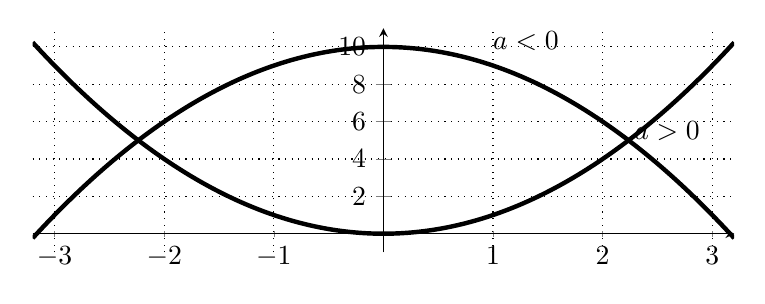
\begin{tikzpicture}
        \begin{axis}[
                xscale=1.3,
                yscale=.5,
                domain=-3.2:3.2,
                axis lines=middle,
                xtick={-3,-2,...,3},
                ytick={0,2,...,10},
                ymin=-1,
                ymax=11,
                clip=true,
                grid style={dotted,black},
                grid=both,
            ]
            \addplot[black, ultra thick, samples=100, smooth]{x^2};
            \addplot[black, ultra thick, samples=100, smooth]{-x^2+10};
            \draw (axis cs:2.2,5.5) node[right]{$a>0$};
            \draw (axis cs:1.3,9.3) node[above]{$a<0$};
        \end{axis}
    \end{tikzpicture}
\end{center}

\Prp[Tableau de variations de $x\mapsto ax^2$]{
\begin{center}
    \begin{minipage}{0.46\linewidth}
        \centering\textbf{Si $a>0$}

        \begin{tikzpicture}
            \tkzTabInit[lgt=2,espcl=2.5]{$x$/1,$f(x)$/2}{$-\infty$,$0$,$+\infty$}
            \tkzTabVar{-/$+\infty$,+/$0$,+/$+\infty$}
        \end{tikzpicture}
    \end{minipage}\hfill
    \begin{minipage}{0.46\linewidth}
        \centering\textbf{Si $a<0$}

        \begin{tikzpicture}
            \tkzTabInit[lgt=2,espcl=2.5]{$x$/1,$f(x)$/2}{$-\infty$,$0$,$+\infty$}
            \tkzTabVar{+/$-\infty$,-/$0$,-/$-\infty$}
        \end{tikzpicture}
    \end{minipage}
\end{center}}

\Prp[Fonctions de la forme $x\mapsto ax^2+c$]{La courbe de $f:x\mapsto ax^2+c$ s'obtient en translatant verticalement celle de $x\mapsto ax^2$ de $c$ unités. Son sommet est le point $S(0\ ;\ c)$, et son axe de symétrie reste l'axe des ordonnées (la droite d'équation $x=0$).}

\Exemple{On considère les fonctions $f:x\mapsto2x^2-3$ et $g:x\mapsto-0,5x^2+4$.
\begin{enumerate}
    \item Donner le sommet et l'axe de symétrie de chacune des deux courbes.

    \textcolor{J1}{Pour $f$ : sommet $S_f(0\ ;\ -3)$, axe de symétrie d'équation $x=0$. Pour $g$ : sommet $S_g(0\ ;\ 4)$, axe de symétrie d'équation $x=0$.}
    \item $f$ et $g$ admettent-elles chacune un minimum ou un maximum ?

    \textcolor{J1}{$f$ admet un minimum, car $a=2>0$ : il est égal à $-3$. $g$ admet un maximum, car $a=-0,5<0$ : il est égal à $4$.}
\end{enumerate}}

\section{Sommet et axe de symétrie de \texorpdfstring{$f(x)=ax^2+bx+c$}{f(x)=ax²+bx+c}}

\Prp{La courbe représentative d'une fonction polynôme du second degré $f:x\mapsto ax^2+bx+c$ est une parabole tournée vers le haut si $a>0$, vers le bas si $a<0$. Elle possède un axe de symétrie vertical, qui passe par le point le plus bas (ou le plus haut) de la courbe, appelé \textcolor{J1}{sommet} de la parabole.}

\ANoter{Contrairement au cas particulier $x\mapsto ax^2+c$, l'axe de symétrie de $f(x)=ax^2+bx+c$ n'est en général plus l'axe des ordonnées : il faut le déterminer.}

\Exemple{\label{ex:sommet}On considère la fonction $f$ définie sur $\R$ par $f(x)=x^2-6x+5$.

\medskip

\textbf{Etape 1} : on remarque que $f(0)=5$, et on cherche un autre nombre $x_0$ tel que $f(x_0)=5$ : son symétrique par rapport à l'axe.\\
\textcolor{J1}{$f(x)=5 \Longleftrightarrow x^2-6x+5=5 \Longleftrightarrow x^2-6x=0 \Longleftrightarrow x(x-6)=0$, donc $x=0$ ou $x=6$. Les points d'abscisses $0$ et $6$ ont donc la même image, $5$.}

\medskip

\textbf{Etape 2} : l'axe de symétrie de la parabole passe par le milieu de ces deux abscisses.\\
\textcolor{J1}{L'axe de symétrie a pour équation $x=\dfrac{0+6}{2}=3$.}

\medskip

\textbf{Etape 3} : le sommet de la parabole est le point de la courbe dont l'abscisse est celle de l'axe de symétrie.\\
\textcolor{J1}{$f(3)=9-18+5=-4$, donc le sommet est le point $S(3\ ;\ -4)$.}

\medskip

\textbf{Etape 4} : comme $a=1>0$, la parabole est tournée vers le haut : $f$ est décroissante jusqu'au sommet, puis croissante.\\
\textcolor{J1}{
\begin{center}
    \begin{tikzpicture}
        \tkzTabInit[lgt=2,espcl=2.5]{$x$/1,$f(x)$/2}{$-\infty$,$3$,$+\infty$}
        \tkzTabVar{-/$+\infty$,+/$-4$,+/$+\infty$}
    \end{tikzpicture}
\end{center}
}

\begin{center}
    \begin{tikzpicture}
        \begin{axis}[
                xscale=1.1,
                yscale=.5,
                domain=-0.5:6.5,
                axis lines=middle,
                xtick={0,1,...,6},
                ytick={-4,-2,...,8},
                ymin=-5,
                ymax=9,
                clip=false,
                grid style={dotted,black},
                grid=both,
            ]
            \addplot[black, ultra thick, samples=100, smooth]{x^2-6*x+5};
            \addplot[only marks, mark=*, J1] coordinates {(3,-4)};
            \draw[J1, dashed] (axis cs:3,-5) -- (axis cs:3,9);
            \draw (axis cs:3,-4) node[right=6pt]{$S(3\,;\,-4)$};
        \end{axis}
    \end{tikzpicture}
\end{center}}

\Exemple{Reprendre la méthode de l'exemple \ref{ex:sommet} pour déterminer le sommet et les variations de $g(x)=-2x^2+8x+1$.

\textcolor{J1}{$g(0)=1$. On résout $g(x)=1 \Longleftrightarrow -2x^2+8x+1=1 \Longleftrightarrow -2x^2+8x=0 \Longleftrightarrow -2x(x-4)=0$, donc $x=0$ ou $x=4$. L'axe de symétrie a pour équation $x=\dfrac{0+4}{2}=2$. Or $g(2)=-8+16+1=9$, donc le sommet est $S(2\ ;\ 9)$. Comme $a=-2<0$, $g$ est croissante jusqu'au sommet, puis décroissante, avec un maximum égal à $9$.}}

\section{Forme factorisée : racines et signe}

\Dfn{Lorsqu'un polynôme du second degré $f(x)=ax^2+bx+c$ s'écrit sous la forme
\[f(x)=a(x-x_1)(x-x_2)\]
on dit qu'il est écrit sous \textcolor{J1}{forme factorisée}. Les nombres $x_1$ et $x_2$ sont alors les \textcolor{J1}{racines} du polynôme, c'est-à-dire les solutions de l'équation $f(x)=0$.}

\ANoter{Retrouver la forme factorisée d'un polynôme du second degré à partir de sa forme développée n'est, en général, pas au programme de cette année (elle fait appel au discriminant) : elle sera le plus souvent donnée dans l'énoncé, ou obtenue par une factorisation simple (facteur commun, identité remarquable).}

\Prp[Résolution par produit nul]{Un produit de facteurs est nul si et seulement si l'un au moins de ses facteurs est nul. Ainsi, les solutions de l'équation $a(x-x_1)(x-x_2)=0$ (avec $a\neq0$) sont exactement $x_1$ et $x_2$.}

\Exemple{Donner les racines du polynôme $f(x)=3(x+2)(x-5)$.

\textcolor{J1}{$f(x)=0 \Longleftrightarrow x+2=0$ ou $x-5=0 \Longleftrightarrow x=-2$ ou $x=5$. Les racines de $f$ sont donc $-2$ et $5$.}}

\Exemple{Factoriser $g(x)=2x^2-8x$ à l'aide d'un facteur commun, puis donner ses racines.

\textcolor{J1}{$g(x)=2x(x-4)$, sous forme factorisée avec $x_1=0$ et $x_2=4$ : ce sont les racines de $g$.}}

\Prp[Signe d'un polynôme du second degré factorisé]{Soit $f(x)=a(x-x_1)(x-x_2)$ un polynôme du second degré factorisé, avec $x_1\leq x_2$. Alors $f(x)$ est :
\begin{itemize}
    \item du signe de $a$ à l'extérieur des racines, c'est-à-dire sur $\left]-\infty\ ;\ x_1\right[$ et sur $\left]x_2\ ;\ +\infty\right[$ ;
    \item du signe opposé à $a$ entre les racines, c'est-à-dire sur $\left]x_1\ ;\ x_2\right[$ ;
    \item nul en $x_1$ et en $x_2$.
\end{itemize}}

\Exemple{Dressons le tableau de signes de $f(x)=-2(x+1)(x-4)$ sur $\R$.

\medskip

\textbf{Etape 1} : on détermine les racines, c'est-à-dire les valeurs qui annulent chaque facteur.\\
\textcolor{J1}{$x+1=0 \Longleftrightarrow x=-1$ \qquad et \qquad $x-4=0 \Longleftrightarrow x=4$.}

\medskip

\textbf{Etape 2} : on applique la propriété précédente, avec $a=-2<0$.

\begin{center}
    \begin{tikzpicture}
        \tkzTabInit[lgt=3,espcl=2.5]
          {$x$ / 1 , Signe de $f(x)$ / 1}
          {$-\infty$, \textcolor{J1}{$-1$}, \textcolor{J1}{$4$}, $+\infty$}
        \tkzTabLine{, \color{J1}-, \color{J1}0, \color{J1}+, \color{J1}0, \color{J1}-, }
    \end{tikzpicture}
\end{center}

\textcolor{J1}{$f$ est donc négative sur $\left]-\infty\ ;\ -1\right]$ et sur $\left[4\ ;\ +\infty\right[$, et positive sur $\left[-1\ ;\ 4\right]$ --- ce qui est cohérent avec $a=-2<0$ (signe de $a$ à l'extérieur des racines, signe opposé entre les racines).}}

\ANoter{Le signe d'un polynôme du second degré renseigne sur la position de sa parabole par rapport à l'axe des abscisses : la courbe est au-dessus de l'axe là où $f$ est positive, en dessous là où $f$ est négative, et coupe l'axe en ses racines.}

% !TEX root = ../PolycopiePremiere2627.tex
%%%%%%%%%%%%%%%%%%%%%%%%%%%%%%%%%%%%%%%%%%%%%%%%%%%%%%%%%%%%%%%%%%%%%%%%%%%%%%%%
% Contenu initial repris de Louis Paternault --- http://ababsurdo.fr
%
% Publié sous licence Creative Commons Attribution-ShareAlike 4.0 International (CC BY-SA 4.0)
% http://creativecommons.org/licenses/by-sa/4.0/deed.fr
%%%%%%%%%%%%%%%%%%%%%%%%%%%%%%%%%%%%%%%%%%%%%%%%%%%%%%%%%%%%%%%%%%%%%%%%%%%%%%%%

\chapter{Suites géométriques}

\noindent\textbf{Activité}

On définit la suite $v$ par le schéma suivant.

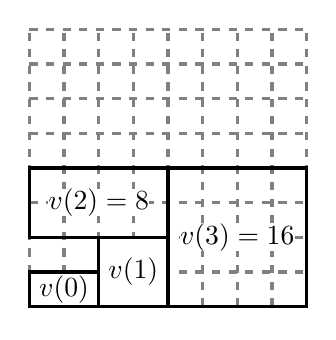
\begin{tikzpicture}[scale=.44,very thick]
    \draw[dashed, gray] (0, 0) grid (8, 8);
    \draw (0, 2) rectangle (4, 4) node[midway, fill=white, inner sep=0pt]{$v(2)=8$};
    \draw (4, 0) rectangle (8, 4) node[midway, fill=white, inner sep=0pt]{$v(3)=16$};
    \draw[fill=white](2, 0) rectangle ++(2, 2) node[midway]{$v(1)$};
    \draw[fill=white](0, 0) rectangle ++(2, 1) node[midway]{$v(0)$};
\end{tikzpicture}%
\begin{minipage}[b]{.7\textwidth}
    \begin{enumerate}
        \item Donner $v(0)$ et $v(1)$.
        \item Quel calcul doit être fait à chaque étape pour calculer le terme suivant ?\\
        \item Calculer :

        \begin{tabularx}{\linewidth}{XXX}
            $v(4)=\ldots$ ;&
            $v(5)=\ldots$ ;&
            $v(7)=\ldots$ ;\\
            $v(25)=\ldots$ ;&
            $v(100)=\ldots$ ;&
            $v(-1)=\ldots$.\\
        \end{tabularx}
        \item Exprimer $v(n+1)$ en fonction de $v(n)$.
    \end{enumerate}
\end{minipage}

\bigskip

Une suite est géométrique si on passe au terme suivant en multipliant (ou divisant) toujours le même nombre.

\Dfn{Une suite $u$ est dite \textcolor{J1}{géométrique} s'il existe un réel $q$, appelé \textcolor{J1}{raison}, tel que pour tout $n\in\mathbb{N}$, on ait : \textcolor{J1}{$u_{n+1}=q\times u_n$}.

Habituellement, une suite géométrique est définie par la donnée de \textcolor{J1}{son premier terme et sa raison}.}

\Exemple[avec calculatrice]{\label{ex:calculGeo}
\begin{enumerate}
    \item Donner les cinq premiers termes (arrondis au centième) de la suite géométrique $u$ de premier terme $u_0=2$ et de raison \numprint{2,5}.
    \item La suite $v$ est géométrique, et on sait que $v_3=2$ et $v_5=18$. Déterminer la raison positive, puis calculer $v_4$, $v_6$, et $v_2$.
\end{enumerate}}

\Exemple{\label{ex:graphGeo}
Représenter graphiquement (de couleur différente) les deux suites de l'exemple \ref{ex:calculGeo}. Les suites sont-elles arithmétiques ?
\begin{center}
    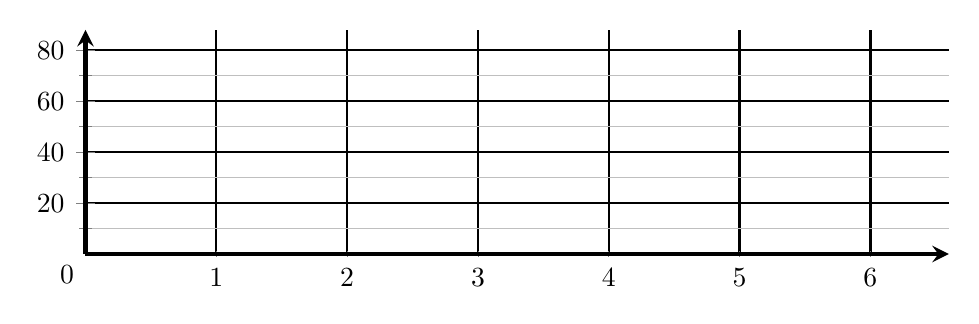
\begin{tikzpicture}[scale=1,very thick]
        \begin{axis}[
                yscale=.5,
                xscale=1.6,
                xmin=0,
                xmax=6,
                ymin=0,
                ymax=80,
                ultra thick,
                axis lines=middle,
                enlargelimits=upper,
                minor y tick num=1,
                major grid style={black, thick},
                grid=both,
                clip=false,
            ]
            \draw (axis cs:0, 0) node[below left]{$0$};
        \end{axis}
    \end{tikzpicture}%
\end{center}}

\Prp{On dit que les termes d'une suite géométrique suivent un modèle de \textcolor{J1}{croissance exponentielle}.}

\pagebreak

\Prp{Une suite géométrique $u$ de premier terme strictement positif est :
\begin{itemize}
    \item \emph{croissante} si et seulement si sa raison est \textcolor{J1}{$q>1$} ;
    \item \emph{décroissante} si et seulement si sa raison est \textcolor{J1}{$0<q<1$} ;
    \item \emph{constante} si sa raison est \textcolor{J1}{$q=1$}.
\end{itemize}}

\Exemple{Déterminer les variations des deux suites $u$ et $v$ de l'exemple \ref{ex:calculGeo}.}

\Prp{
\begin{itemize}
    \item Pour tout $n$ et $p$ de son domaine de définition, on a : \[\textcolor{J1}{u_n=u_p\times q^{n-p}}\]
    \item En particulier, si $u$ est définie sur $\mathbb{N}$, pour tout $n\in\mathbb{N}$, on a : \[\textcolor{J1}{u_n=u_0\times q^n}\]
\end{itemize}}

\Exemple{On reprend les suites $u$ et $v$ de l'exemple \ref{ex:calculGeo}. Sans utiliser le module suite de la calculatrice, déterminer $u_{100}$ et $v_{100}$.}

\Exemple[D'après le sujet zéro de l'épreuve anticipée de mathématiques aux baccalauréats général et technologique 2026]{
Victor sort un plat du four. La température du plat est alors égale à 180\,\textdegree C. Il place ce plat dans une pièce dont la température est égale à 25\,\textdegree C. Le plat refroidit.

Le plat ne pourra être servi que lorsque sa température sera devenue inférieure ou égale à 40\,\textdegree C.

Trois minutes après la sortie du four, on mesure que la température du plat est égale à 105\,\textdegree C.

Pour tout entier naturel $n$ on note $U_n$, la différence entre la température du plat et la température de la pièce, $n$ minutes après la sortie du four.

Exemple : 3 minutes après la sortie du four, l'écart avec la température de la pièce est égal à $105 - 25 = 80$. On a donc $U_3 = 80$.

\begin{enumerate}[wide=0pt]
    \item Justifier que $U_0 = 155$.
    \item On suppose que chaque minute la différence $U_n$ diminue de 20\%.
    \begin{enumerate}[wide=0pt]
        \item Justifier que, pour tout entier naturel $n$, on a $U_{n+1} = 0,8U_n$.
        \item En déduire la nature de la suite $(U_n)$ et donner sa raison.
        \item Exprimer $U_n$ en fonction de $n$, pour tout entier naturel $n$.
        \item On dispose des données suivantes (arrondies à $10^{-1}$). Au bout de combien de minutes, Victor pourra-t-il servir le plat ?
        \[\begin{array}{*{14}{c}}
            \hline
            n & 3 & 4 & 5 & 6 & 7 & 8 & 9 & 10 & 11 & 12 & 13 & 14 & 15 \\
            \hline
            U_n & 80 & 64 & 51,2 & 41 & 32,8 & 26,2 & 21 & 16,8 & 13,4 & 10,7 & 8,6 & 6,9 & 5,5 \\
            \hline
        \end{array}\]
    \end{enumerate}
\end{enumerate}}

% !TEX root = ../PolycopiePremiere2627.tex
%%%%%%%%%%%%%%%%%%%%%%%%%%%%%%%%%%%%%%%%%%%%%%%%%%%%%%%%%%%%%%%%%%%%%%%%%%%%%%%%
% Contenu initial repris de Louis Paternault --- http://ababsurdo.fr
%
% Publié sous licence Creative Commons Attribution-ShareAlike 4.0 International (CC BY-SA 4.0)
% http://creativecommons.org/licenses/by-sa/4.0/deed.fr
%%%%%%%%%%%%%%%%%%%%%%%%%%%%%%%%%%%%%%%%%%%%%%%%%%%%%%%%%%%%%%%%%%%%%%%%%%%%%%%%

\chapter{Fonction exponentielle}

\noindent\textbf{Activité}

En un an, le nombre d'abonnés d'une chaîne de vidéos sur un réseau social a augmenté de 30\%. Quel a été le taux d'évolution moyen par mois tout au long de cette année ?

\section{Fonction exponentielle}

\Dfn{On appelle \emph{fonction exponentielle} de base $a$ (où $a$ est un nombre réel strictement positif) la fonction $f$ définie sur $\R$ par $f:x\mapsto a^x$.}

\Prp[Règles de calcul]{Pour tous nombres réels $a$ et $b$ strictement positifs, et tous nombres $x$ et $y$ réels, on a :
\begin{multicols}{2}
\begin{enumerate}[label=(\roman*)]
    \item $a^0=1$
    \item $a^x\times a^y=a^{x+y}$
    \item $\left( a^x \right)^y=a^{x\times y}$
    \item $a^x\times a^{-x}=1$
    \item $a^{-x}=\dfrac{1}{a^x}$
    \item $a^{x-y}=\dfrac{a^x}{a^y}$
    \item $\left(a \times b\right)^x=a^x\times b^x$
\end{enumerate}
\end{multicols}}

\Exemple{Simplifier autant que possible les expressions suivantes :
\begin{enumerate}
    \item $3^{2,5}\times3^{-2}=$
    \item $\dfrac{5^{7}}{5^{2}}=$
    \item $\dfrac{2^{2,5}\times2^{3,5}+\left(2^{1,5}\right)^4}{7,6^0\times2^{4}}=$
\end{enumerate}}

\Prp[Sens de variations]{Soient $k$ et $a$ deux nombres strictement positifs, et $f$ la fonction définie sur $\R$ par $f(x)=k\times a^x$. Alors :
\begin{itemize}
    \item si $0<a<1$, alors la fonction $f$ est strictement décroissante sur $\R$ ;
    \item si $a=1$, alors la fonction $f$ est constante sur $\R$ ;
    \item si $a>1$, alors la fonction $f$ est strictement croissante sur $\R$.
\end{itemize}}

\Exemple{Dresser le tableau de variations de la fonction $f$ définie par $f(x)=4\times\pi^x$.}

\Prp[Courbe représentative]{
\begin{center}
    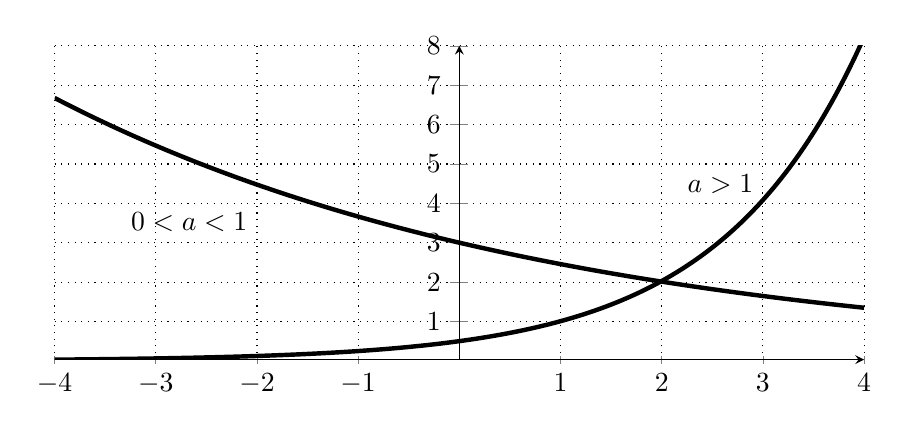
\begin{tikzpicture}
        \begin{axis}[
                xscale=1.5,
                yscale=.7,
                domain=-4:4,
                axis lines=middle,
                xtick={-4, -3, ..., 4},
                ytick={1, 2, ..., 8},
                ymax=8,
                clip=true,
                grid style={dotted,black},
                grid=both,
            ]
            \addplot[black, ultra thick, samples=100,smooth]{.5*exp(.7*x)};
            \addplot[black, ultra thick, samples=100,smooth]{3*exp(-.2*x)};
            \draw (axis cs:-2, 4) node[below left]{$0<a<1$};
            \draw (axis cs:3, 4) node[above left]{$a>1$};
        \end{axis}
    \end{tikzpicture}
\end{center}}

\Exemple{Associer chacune des fonctions suivantes à sa courbe.
\[\begin{array}{*{4}{c}}
    f(x)=3^x&
    g(x)=2\times\left(^1/_3\right)^x&
    h(x)=3\times2^x&
    k(x)=3\times0,5^x\\
\end{array}\]

\begin{center}
    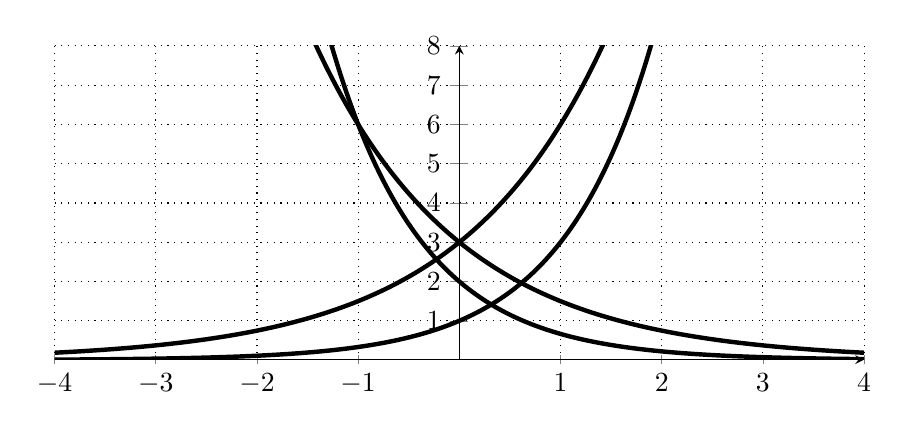
\begin{tikzpicture}
        \begin{axis}[
                xscale=1.5,
                yscale=.7,
                domain=-4:4,
                axis lines=middle,
                xtick={-4, -3, ..., 4},
                ytick={1, 2, ..., 8},
                ymax=8,
                clip=true,
                grid style={dotted,black},
                grid=both,
            ]
            \addplot[black, ultra thick, samples=100,smooth]{1*3^x};
            \addplot[black, ultra thick, samples=100,smooth]{2*.33333^x};
            \addplot[black, ultra thick, samples=100,smooth]{3*2^x};
            \addplot[black, ultra thick, samples=100,smooth]{3*0.5^x};
        \end{axis}
    \end{tikzpicture}
\end{center}}

\section{Racine $n$-ième}

\Prp{Pour tout nombre $a$ positif, l'équation $x^n=a$ admet une unique solution réelle positive : $x=a^{^1/_n}$.}

\Exemple{Résoudre les deux équations suivantes (arrondir au centième).
\begin{enumerate}
    \item $x^4=8$
    \item $4x^7=5x$
\end{enumerate}}

\Exemple{Une biologiste a laissé des bactéries se reproduire pendant exactement 24 heures, et elle a observé que le nombre de ces bactéries a été multiplié par 4. Quel a été le taux d'évolution moyen du nombre de ces bactéries, par heure ?}


\end{document}
